\startchapter{Method}
\label{chapter:method}
I conducted a user study based on a repetitive task consisting of grab and
release actions.  
For each task, data describing the state of users' hands and the experiment interface were logged.  
These data logs were then analyzed to suggest parameters that would reliably
predict center of action as well as other interesting information about the
action, such as which hand was used to perform it.

\section{Study Design}
Two independent variables were studied: position and size of object and target.
Positions were generated randomly within a predefined square region inside the screen with the resolution of 1600 by 900.  Sizes were generated randomly between 20 and 500 pixels which span the range of 0.5 cm to 13.5 cm.  The four empirically tested models used a total of \textit{eight} dependent variables: 
\begin{itemize}
 \item \textbf{(CC)} \textit{center position} and \textit{radius} of the minimum enclosing circle
 \item \textbf{(RC)} \textit{center position}, \textit{size} and \textit{angle} of the minimum enclosing rectangle
 \item \textbf{(FM)} \textit{mean} and \textit{standard deviation} of feature position
 \item \textbf{(MC)} \textit{position} of the center of mass
\end{itemize}
Because even slight system errors and inconsistencies can negatively impact a participant's performance or lead to undesired subconscious learning, I used a Wizard of Oz approach to classify user actions.  
This Wizard of Oz classifier was used to create a system that was nearly 100\% accurate and enabled us to negate the classifier as a significant source of data noise in my models.

\section{Participants}
Twenty six paid participants (7 female, 19 male), were individually tested in a study that took approximately 30 minutes to complete.  Their ages ranged from 20-44 years (\textit{M} = 27, \textit{SD} = 5.17).  
24 participants were right handed, one participant was left handed, and one participant was ambidextrous.  Twenty of the participants reported using at least one touch enabled device regularly.

\section{Apparatus}
During the study, participants sat on a non-adjustable, fixed chair placed in front of the display as shown in figure \ref{fig:participant_example}.
The angle between the display and the horizontal plane was $60\degree$; the height of the display from the ground to the bottom edge was 75 cm; and, 
the experiment was performed indoors under uniform, controlled lighting conditions.
The display used within the prototype near touch system was a $23in$ (or approximately $51x28 cm$) LED-LCD with a resolution of $1920x1080$ and an aspect ratio of $1.77$.

\begin{figure}[h]
 \centering
 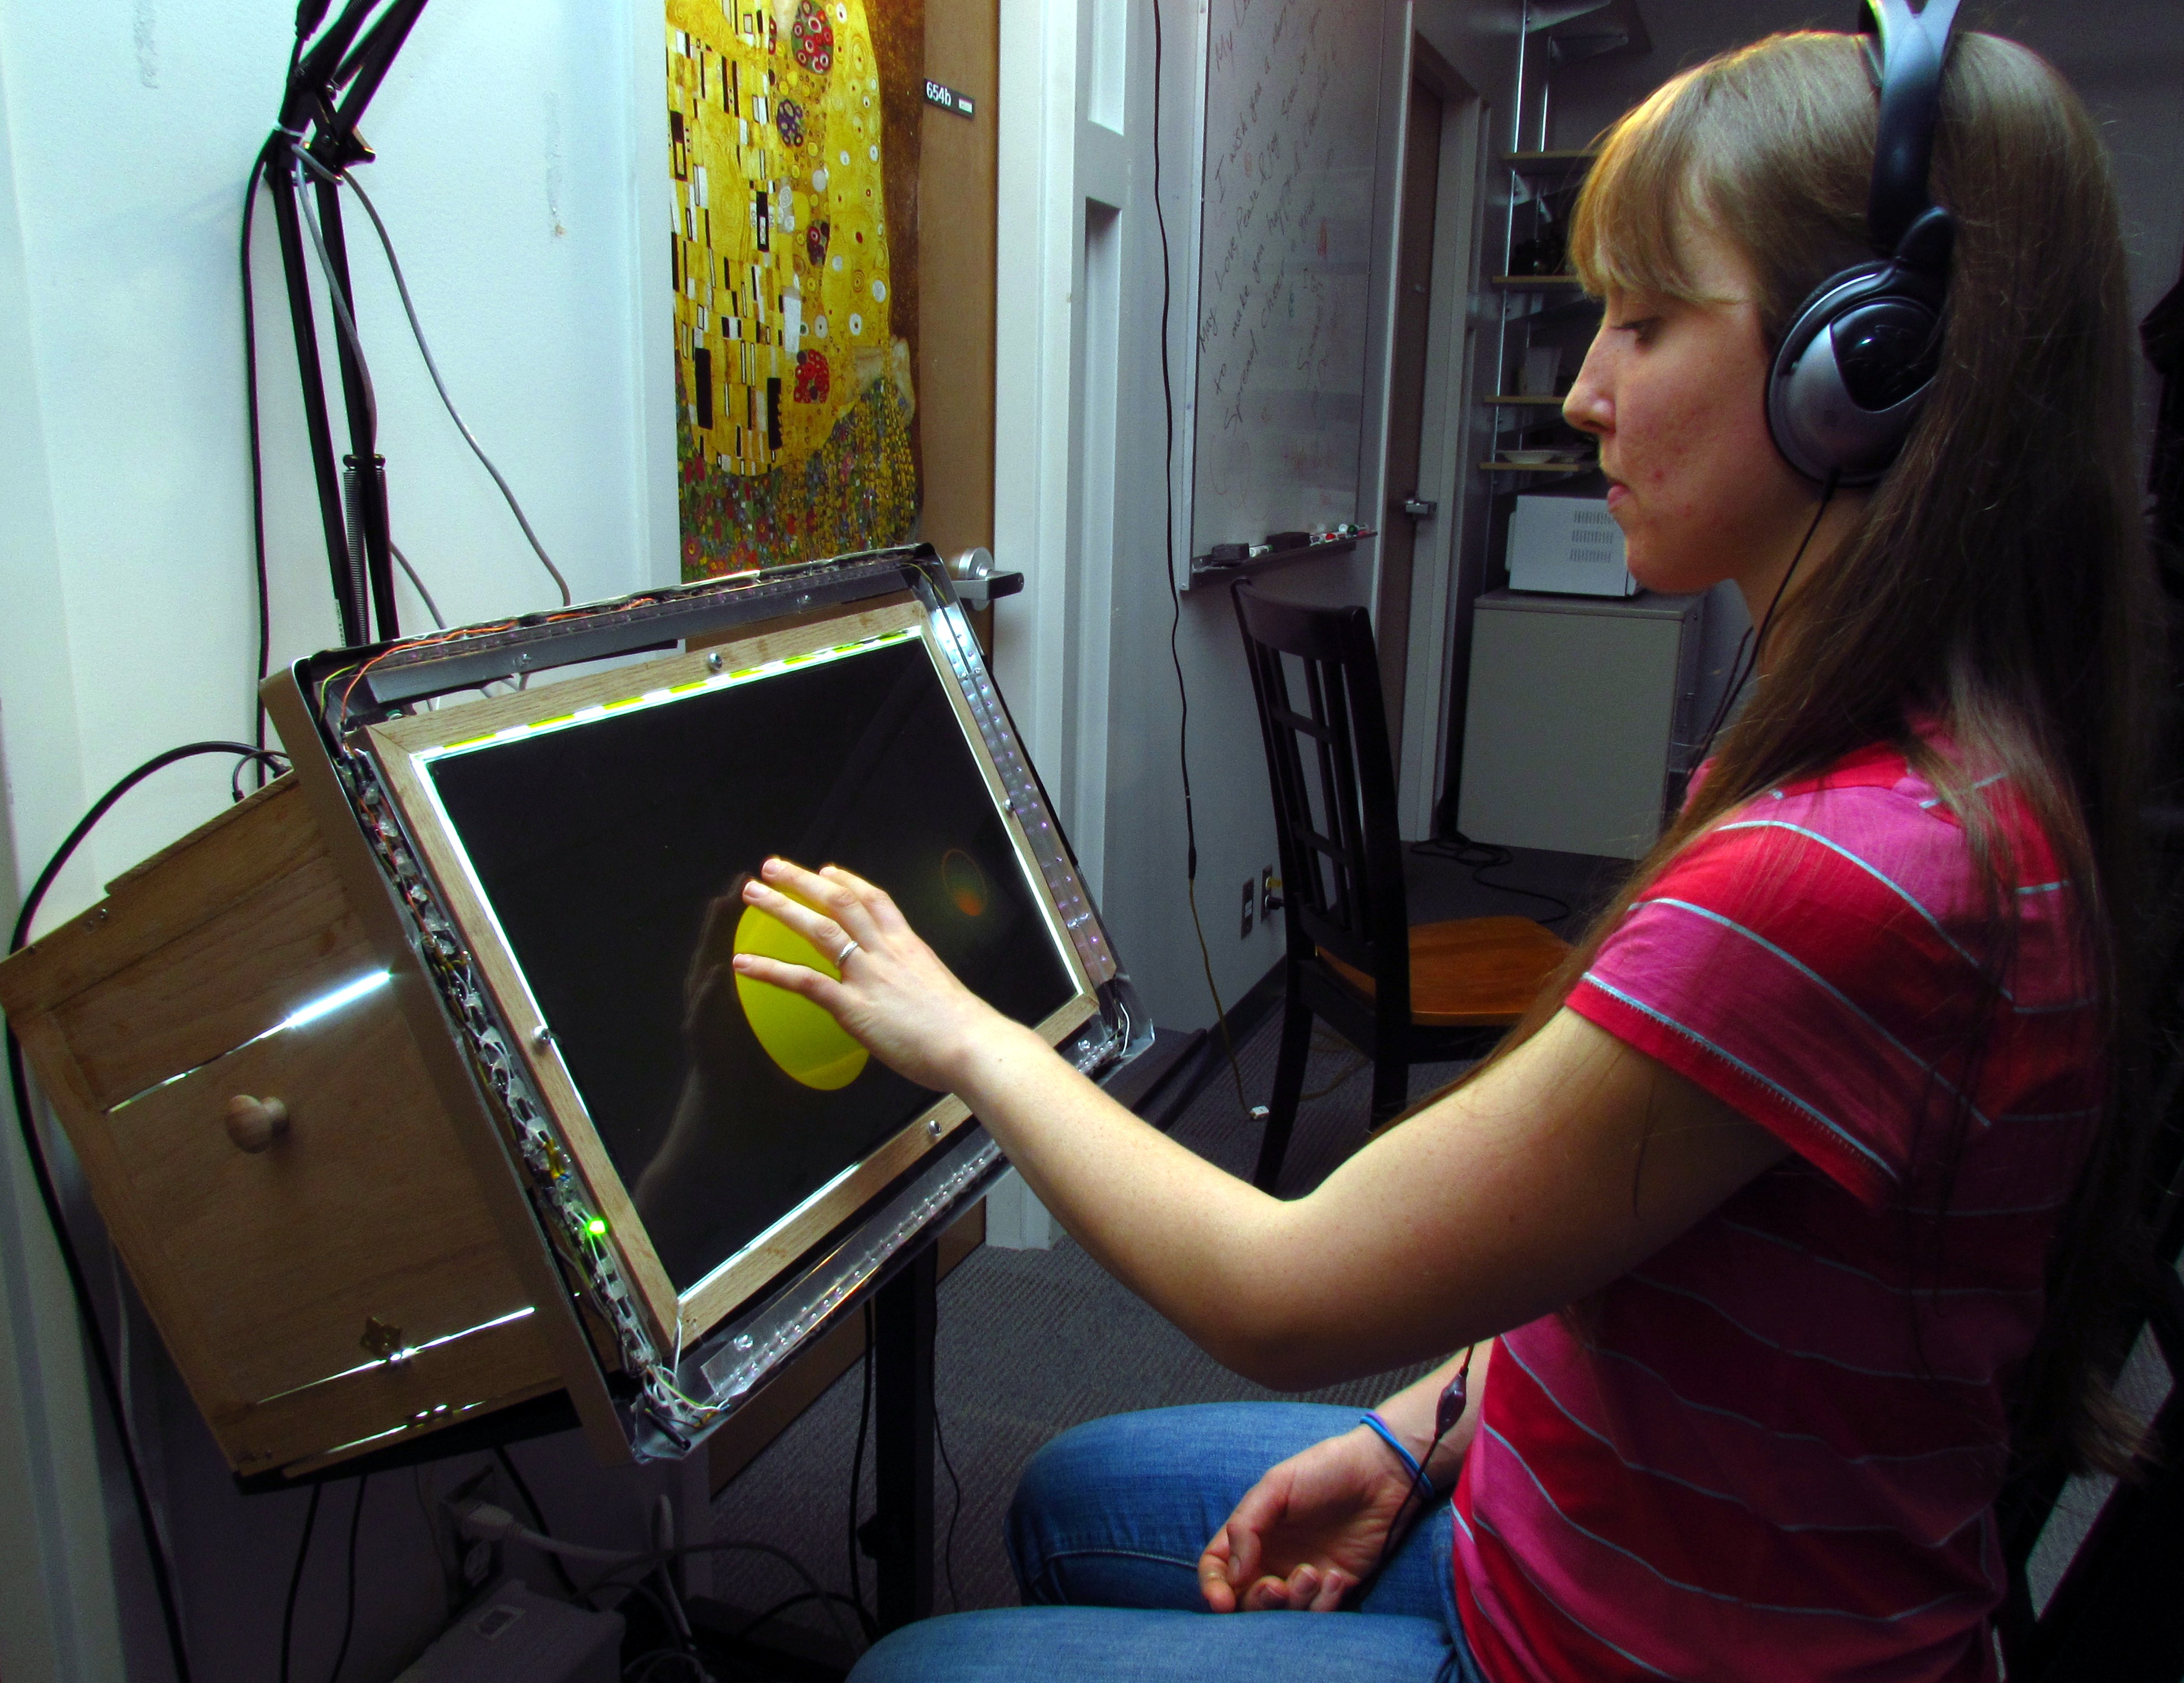
\includegraphics[type=pdf,ext=.pdf,read=.pdf,width=3in]{./img/participant_example}
 \caption[A participant about to perform a grab action on the prototype interface]{
A participant about to perform a grab action on the prototype interface. 
Once the action is performed the yellow circular object will fade away and the target will be highlighted.
A short distinct sound is given after the participant performs either the grab or release action. 
}
 \label{fig:participant_example}
\end{figure}

\subsection{System Hardware}
Typical contemporary multi-touch hardware technologies, such as resistive and capacitive touch screens, do not capture any information about the state of the hand above the surface and are not suitable for this study.
A number of computer vision based techniques for building multi-touch interfaces have existed for several years \cite{Han:2005:LCMTSTFTIR}.
The ultimate goal in the construction of most of these interfaces is to optimize tracking of finger touches on the display surface.  Because these systems typically use infrared illumination and video processing techniques that filter away most of a user's hand from the picture, such techniques are unsuitable for my goal of processing whole-hand near touch interactions. 

Figure \ref{fig:neartouch_prototype} summarizes the components of my prototype system that accomplishes the empirical study goals.  
My prototype uses a high resolution LCD screen and a rear mounted infrared camera.
The primary difference between my prototype and existing camera based interactive surface designs is in the illumination.
Instead of optimizing illumination for extracting touch information, I fully illuminate the hand using an array of 72 infrared LEDs mounted just above the edges of the display as shown in figure \ref{fig:neartouch_prototype}. 
The LEDs have a $5mm$ diameter and produce $940 \pm 40 nm$ infrared light.
Motamedi \cite{motamedi:2008:HTMOSHDTV} has performed a similar experiment and
reported that by modifying the threshold algorithm, the system would be able to
see the hovering hand and that further analysis of this gray-scale image could
determine the distance of the hand from the screen.
As a result, hands are captured by the camera up to $25cm$ away from the screen.
A soft light diffuser with diffusion angle of $15\degree$ is placed under the LCD screen.
The addition of the diffuser improves the quality of the image displayed, as well as providing a medium for capturing the depth of features recognized by the camera.

Algorithm 1 is used to calculate the relative distance of each identified feature from the display.
This algorithm takes advantage of the fact that objects closer to the diffuser become sharper.
The depth value calculated in this way also allows us to reliably distinguish touch from hovering fingers.

\subsection{Tracking Software}
I developed two software applications for the purpose of running this study: a computer vision based tracker and an interactive interface.
Both software applications were executed on the same machine running an Ubuntu Linux 11.10 64 bit operating system.

To develop the tracking software I used the OpenCV computer vision library.
The source code for my tracking software can be forked from https://github.com/arasbm/Gibbon.
This software is capable of simultaneously tracking two hands, extracting their features, and finding fingertips and their relative distance to the screen. 
The distance of fingers to the screen is computed using an algorithm based on image sharpness around the fingertip. 
This value is used to distinguish touch from hovering hands or fingers.
The tracker communicates to interactive client applications using the TUIO (Tangible User Interface Objects -- see tuio.org) protocol and my custom defined messages.

\subsubsection{Calibration}
The tracking software required the following one-time calibration process that suited the needs of all study participants.
Calibration was done using OpenCV's built-in undistortion algorithm using a printed chessboard.
A $16x23cm$ chess board with 8 horizontal and 6 vertical squares was placed on the screen at different locations and registered by the system 6 times.
As a result the calibrated input image closely mirrors what actually is in front of the screen.

\subsubsection{Preprocessing}
After applying calibration, each frame retrieved from the camera was preprocessed using two filters which are explained below.
First, a copy of the image was converted to binary using a threshold value of $T_{noise} = 30$.
This binary image was used to find the contour of the hand.
The shape of this contour is the basis for three of the models for the center of action that presented in this paper (CC, MC, and RC).
Second, a median filter using $width = 9$ was applied to the original copy of the image after calibration.
The median filter replaces each pixel in the image with median of its neighboring pixels that would fit inside a $9\times9$ matrix around that pixel.
The purpose of the median filter is to reduce salt and pepper noise which can be described as very bright or very dark pixels randomly distributed in each frame.
After this preprocessing, the image is passed through feature tracking algorithm to identify and track prominent features in the image.
Each feature is a $26\times26$ matrix that is found using a feature detection algorithm provided by OpenCV (Open Source Computer Vision) library called \textit{GoodFeaturesToTrack}.

\subsubsection{Feature Depth Calculation}
Consider $F$ to be the gradient matrix representing a feature.
This matrix is used to calculate sharpness and consequently relative depth of the feature as shown in algorithm 1 below.
This algorithm works by first calculating the minimum eigenvalue of a
% $16\times16$ 
matrix around each pixel in $F$.
This data is achieved by using OpenCV \textit{CornerMinEigenVal} function and stored in a new matrix $S$.
Finally, obtain average of all values in $S$ which gives a single value representing sharpness of the feature.
Because of properties of the diffuser and the way it is used in construction of the hardware prototype, this sharpness value also represents relative distance of the feature from the screen.

\begin{algorithm}[h]
\begin{algorithmic}
\item$F$ \Comment{Matrix representing a feature}
\item$S$ \Comment{Matrix to store minimum eigenvalues corresponding to each element in $F$}
\item$D$ \Comment{Relative depth of feature -- to be calculated}
%\State $S \gets 0$ \Comment{Initialize all elements of $S$ to zero}
\For{$S_i \in S$ }
    \State $T$ \Comment{Obtain a new gradient matrix centered at $S_i$}
    \State $S_i \gets \lambda_{min}(T)$ \Comment{Assign minimum eigen value of $T$ to $S_i$}
\EndFor
\State $D \gets 1/N \sum_i S$ \Comment{Average all elements in $S$}
\State \Return $D$
\end{algorithmic}
\caption{A method for detecting relative depth of a feature based on its sharpness}
\end{algorithm}

\subsection{Interaction Software}
The interaction software is an application that is independent from the tracking software.
It is written in python using the Kivy framework \cite{Kivy:2012:homepage}, which has built-in components for receiving TUIO messages.
Figure \ref{fig:experiment_ui} shows the characteristics of the experiment user interface.
\begin{figure}
\centering
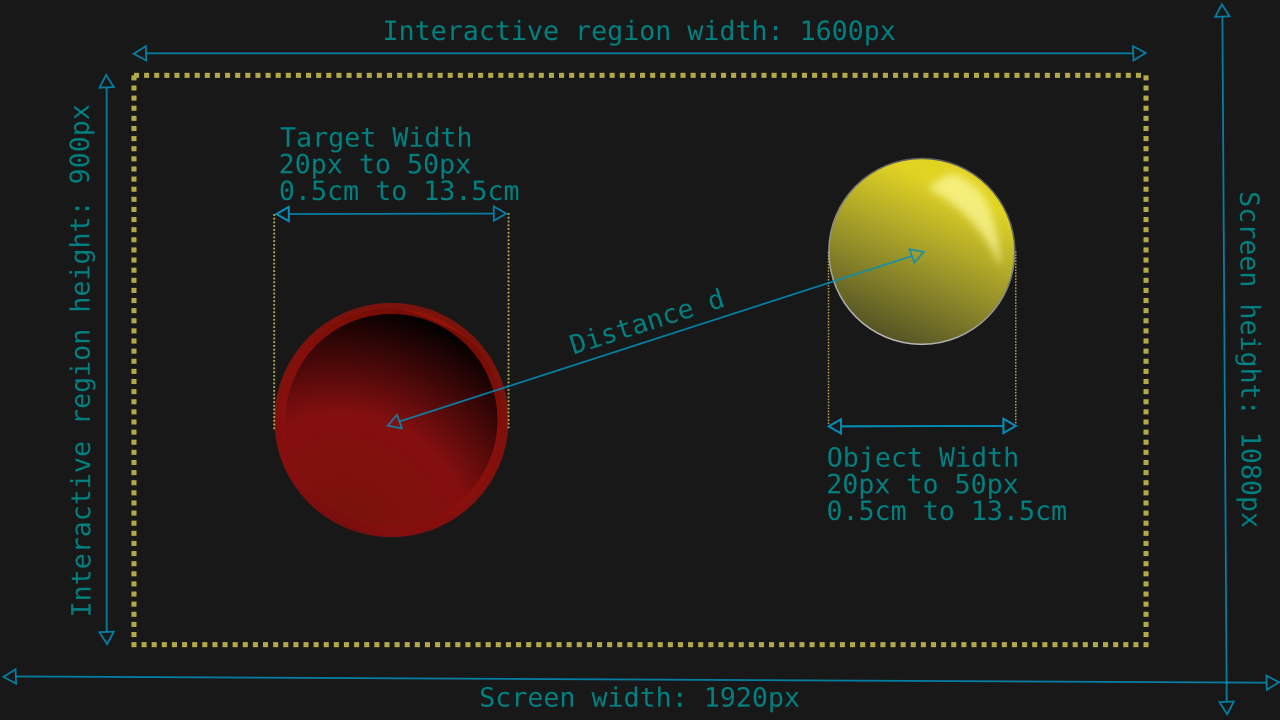
\includegraphics[type=pdf,ext=.pdf,read=.pdf,width=3in]{./img/inprogress/experiment_ui.png}
\caption[The interactive user interface used in the experiment.]{
The interactive user interface used in the experiment. 
For each trial, an object and a target were displayed on the screen at random positions within the interaction region.
The algorithm for positioning targets and objects ensured no collisions occurred, and the edges of the screen were excluded to avoid potential issues with image recognition and to have a full image of the hand in every trial.  Shading was chosen based on informal pilots to minimize object vs. target confusion during grab and release actions.
}
\label{fig:experiment_ui}
\end{figure} 

\section{Procedure}
The study used a targeting task involving grabbing an object and then releasing it on a target.  
In each trial, the participant was presented with an object and a target, both circular but colored differently as shown in Figure \ref{fig:experiment_ui}.  
At the beginning of a trial, the object was highlighted with a higher opacity than the target.  
Once the participant grabbed the object, a short sound was played and then the target was highlighted.
When the participant released the object on the target, another sound was played and the screen was cleared in preparation for the next trial.
I minimized biasing the participants by purposely not informing them that I was studying the center of their hand placements.  
Details of the study design, such as the Wizard of Oz approach, were also hidden from the participants.  

After greeting participants, the study purpose was briefly explained as an exercise to understand two actions called grab and release and to find how a computer system can detect these actions.
I used a printed sheet of paper to show a sample object and target of the study interface.
Using the piece of paper, participants were first shown an example and then given the opportunity to practice the actions of grab and release without system feedback.
I was careful not to give the participants any special instructions as how exactly to perform grab or release actions.
It was expected that there will be variations in the participants' way of
performing grab and release actions.
If a user asked how many fingers they should use to perform grab or release, I
would tell them to perform the action in any way they are more comfortable.
During the study participants prominently used anywhere between 2 to 5 fingers for performing the actions.
Furthermore, it was explained to the participants that:
\begin{itemize}
 \item You can perform actions in whichever way you prefer or find most comfortable.
 \item The interface is capable of tracking your hand near the surface or on the surface. You do not have to touch the surface when you are performing the actions. However if you do touch the screen, that does not interfere with the task.
 \item You can perform the tasks with either hand and you can switch hands at any time during the study, but I ask that you only use one hand at a time on the interface.
 \item Please perform the tasks as quickly and accurately as possible.
\end{itemize}

After the introduction, participants were given a brief background questionnaire.
To begin the study, participants were instructed to sit in front of the prototype and put on a set of headphones to block any distracting ambient sounds and to hear the sound feedback to each trial.
Figure \ref{fig:participant_example} shows a participant as she is about to perform a grab action on my prototype.
Each participant first performed 20 practice trials to become comfortable with the study prototype and trial task.  The data from practice trials were not analyzed.
The participant then performed 400 trials in two sessions (200 each), taking a five minute break between sessions.  Object and target positions were randomized for each trial.
\begin{figure}[h]
 \centering
 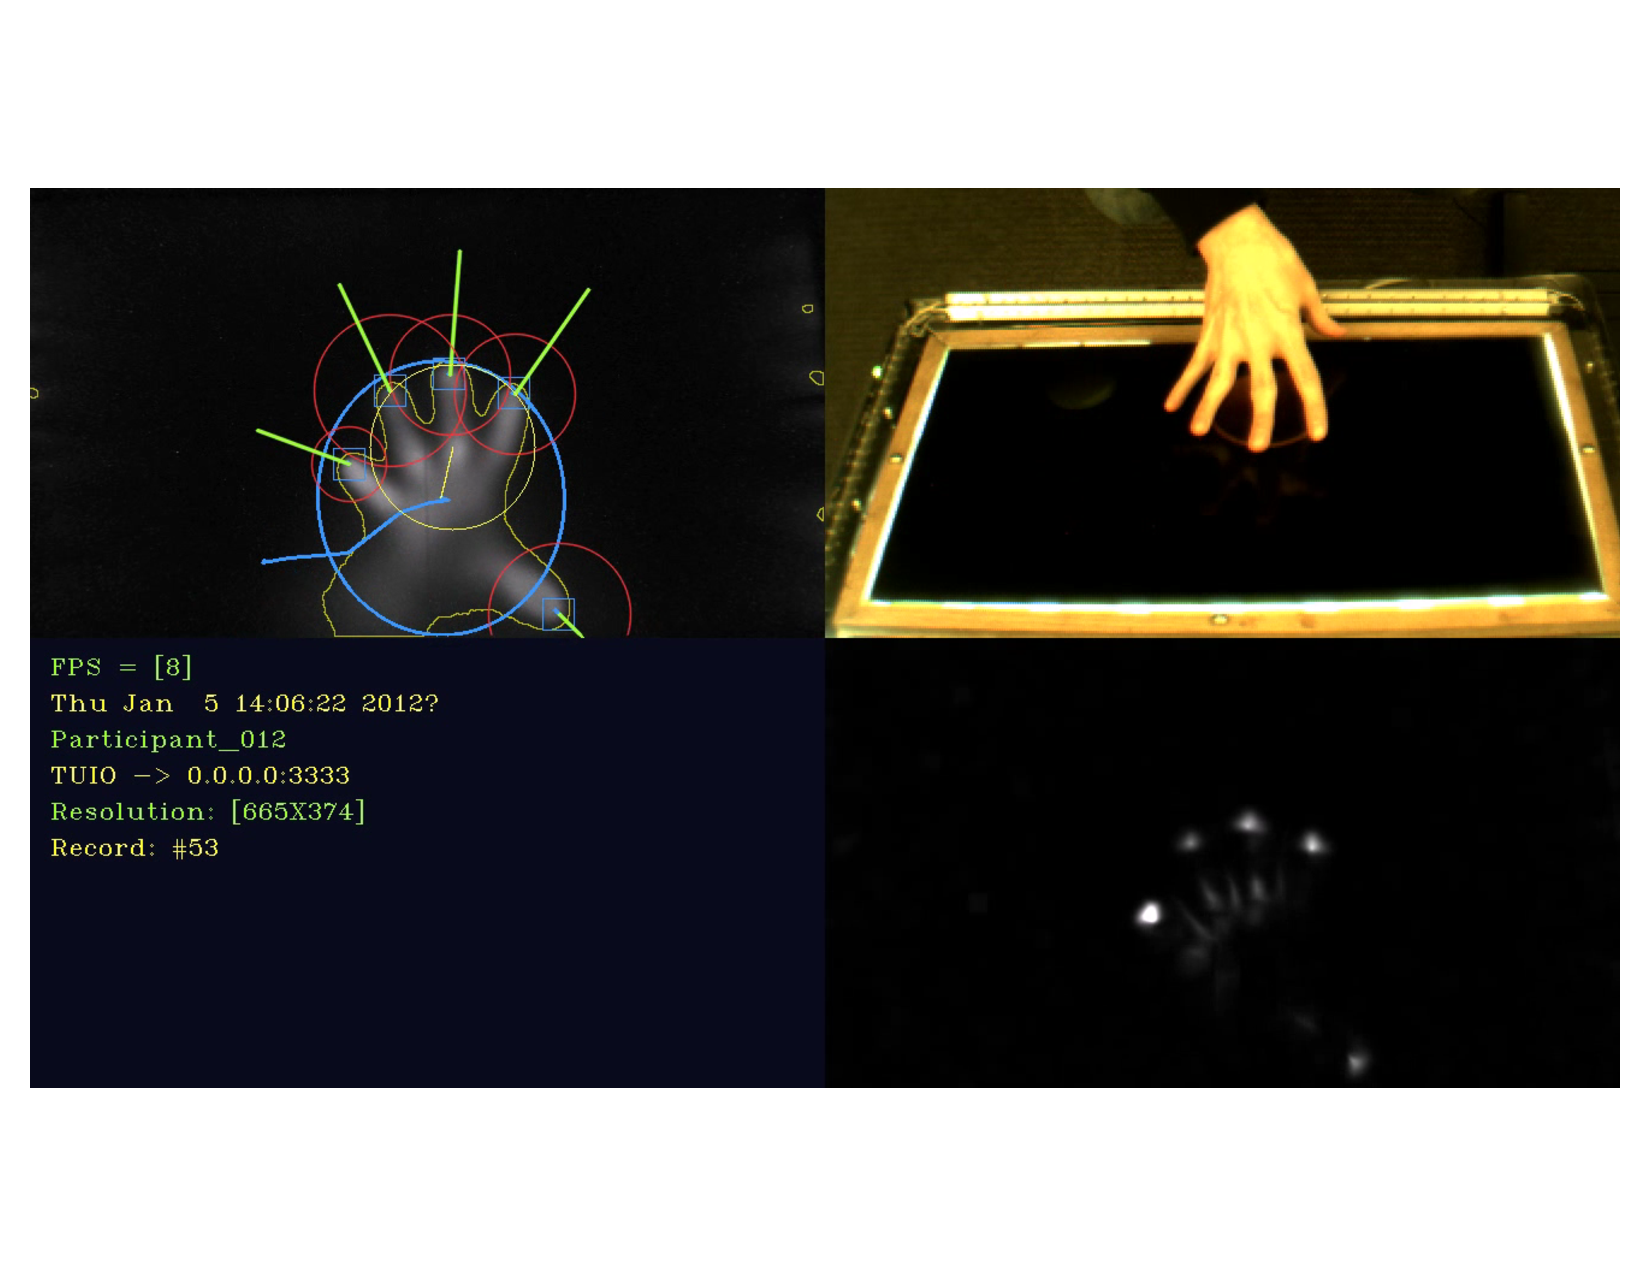
\includegraphics[type=pdf,ext=.pdf,read=.pdf,width=5in]{./img/woz_screenshot}
 \caption[Example Wizard of Oz screen.]{
Example Wizard of Oz screen.
The wizard is able to anticipate participant actions by viewing the overhead camera video (top right).
Near touch and contact interactions can be viewed with the hand video (top left) and intermediate sharpness video (bottom right).
Logging actions can be monitored on the record screen (bottom left).
Actions were registered by pressing either the \textit{J} or \textit{K} key on the keyboard.
}
 \label{fig:woz_example}
\end{figure}
A human wizard was in charge of detecting and sending commands corresponding to grab and release actions, while the system simultaneously tracked a user's hand.
Figure \ref{fig:woz_example} shows an example Wizard of Oz screen viewed by the wizard.
For each action detected by the wizard, the system stored a record describing the shape, features, and position of the hand for twelve frames.
The object size and location, target size and location, participant number, and time of action were also appended to each record.
Each trial included two records, one for grab and one for release. 

After the study, users were given a brief questionnaire.  
Participants were asked to rate fatigue on a multiple choice scale and then provide open-ended comments suggesting (i) any new actions that they thought should be detected by a future system, (ii) interaction ideas based on grab and release actions, and (iii) other general comments.

\section{Data Collection}
For the purpose of the current experiment three log files were recorded in real
time -- two files by tracking software and one by the experiment user interface.
The tracking software identifies features of the hand and records several
attributes of each feature and additional data about the state of the hand such
as contour of the hand in a CSV (comma separated values) file.
Additionally, all the available parameters are stored redundantly as a feature matrix in a second file using the YAML (YAML Ain't Markup Language) format.
The purpose of this second file is to store descriptive parameters in a format that is suitable for training algorithms.
This data was stored with the hope that in future myself or someone else could use it to train classifier algorithms for grab and release actions.
The third log file was stored by the experiment user interface in a CSV (comma separated values) format.
This file contains parameters about the state of the application interface when an action message was received.

At the time of designing the study and developing the experiment software, it was not known which attributes would play an important role in modeling center of action, therefore I decided to collect any attributes of features and other descriptive parameters based on image of the hand that I suspected may have an effect on models for the center of action.
The choice for including these parameters is based on my initial observation of users during pilot studies and the availability of the parameters when developing the tracking software.
The log files were combined after each session into one larger data file based on matching record number and time stamp.
Each record in the combined data contains all the data collected during a
temporal window just before either a grab or a release actions was detected.
Table \ref{table:data_parameters} shows a list of all relevant fields in the combined data file and sample values that were used during the analysis and modeling process.
Other parameters that were also stored but not used during the modeling process include:
\begin{itemize}
 \item 10 Spatial and central image moments which are standard statistical properties of an image
 \item Position of each feature at every frame within the temporal window
 \item Vector describing moving direction and speed of each feature
 \item Relative depth value for each feature calculated using Algorithm 1 based on image sharpness
\end{itemize}
\begin{center}
\begin{table}
\centering
\label{table:data_parameters}
\caption{List of parameters stored by the tracking system and experiment user interface that were used in the study. 
This list includes an example record and description of parameters.}
\begin{tabular}{|l p{2cm} p{9cm}|}
\hline
Parameter & Example & Description \\
\hline
$participant\_number$ & 20 & 1 to 26 \\
$part$ & 1 & 1 or 2 -- each participant performed the experiment twice \\
$record\_number$ & 82 & counted by tracker and reset to 0 for each part \\
$frame\_number$ & 1696 & reset to 0 for each part performed by a participant \\
$hand\_number$ & 0 & 0 for left and 1 for right\\
$action\_type$ & grab & either ``grab'' or ``release''\\
$time\_stamp$ & Fri Jan  6 12:48:04 2012 & end of temporal window, calculated by tracker\\
$fps$ & 9 & number of frames per second being processed\\
\hline
\multicolumn{3}{|c|}{The fields below were repeated 12 times -- once for each frame}\\
\hline
$min\_rect.center.x$ & 495.546 & X position of minimum enclosing rectangle\\
$min\_rect.center.y$ & 174.59 & Y position of minimum enclosing rectangle\\
$min\_rect.size.width$ & 277.155 & width of the minimum enclosing rectangle\\
$min\_rect.size.height$ & 119.426 & height of the minimum enclosing rectangle\\
$min\_rect.angle$ & -71.9958 & the angle of rectangle between $-90\degree$ and
$90\degree$\\
$min\_circle.center.x$ & 497.5 & X position of the minimum enclosing circle\\
$min\_circle.center.y$ & 177.5 & Y position of the minimum enclosing circle\\
$min\_circle.radius$ & 141 & radius of the minimum enclosing circle\\
$mass.center.x$ & 501.903 & X position of center of mass for the contour of the hand\\
$mass.center.y$ & 166.845 & Y position of center of mass for the contour of the hand\\
$feature\_mean.x$ & 543.737 & Average X coordinate of features\\
$feature\_mean.y$ & 92.0414 & Average Y coordinate of features\\
$feature\_StdDev$ & 13.5157 & Standard deviation of features\\
$num\_of\_features$ & 5 & number of features between 0 and 5\\
\hline
\multicolumn{3}{|c|}{The following fields were stored from experiment UI (user
interface)}\\
\hline
$record\_number$ & 82 & counted by experiment UI, should match the tracker record number\\
$datetime$ & 2012/01/06 12:48:04.143 & time stamp of when action message was received by UI\\
$trial\_duration$ & 00:00:02.159 & time taken since displaying an object until an action is performed\\
$action\_type$ & grab & action type as expected by the experiment UI \\
$actual\_x\_position$ & 1188.375 & X position of object or target as set by UI\\
$actual\_y\_position$ & 544.655 & Y position of object or target as set by UI\\
$object\_size$ & 153 & size of grab or release object: $20px$ to $500px$\\
\hline
\end{tabular}
\end{table}
\end{center}

I had included simple descriptors for the shape of hand image such as center of mass and minimum enclosing rectangle and circle, therefore I decided not to include spatial and central image moments to reduce redundancy in the models.
Alternatively, one could use image moments instead of those parameters proposed in this study and I suspect they will obtain very similar results in terms of accuracy of models for predicting center of action.
Location of feature mean combined with standard deviation of features sufficiently capture spacial properties of features in case of grab and release actions, therefore I did not include position and relative depth of individual features in the modeling phase.